\documentclass[11pt]{article}
\usepackage{jheppubmod}
\pdfoutput=1
\usepackage{psfrag}
\usepackage{array}
\usepackage{amssymb}
\usepackage{amsmath}
\usepackage{amsthm}
\usepackage{mathtools}
\usepackage{graphicx}
\usepackage{placeins}
\usepackage{xcolor}
\usepackage{mathtools}
\usepackage{amssymb}
\usepackage[labelsep=quad]{subcaption}
\usepackage{hyperref}
\usepackage[T1]{fontenc}
%\usepackage{epstopdf}
\let\normalcolor\relax
\usepackage[square,sort&compress,numbers]{natbib}


% MARCROS

\title{Stock price prediction}
\author{Pushkal Shrivastava}
%\affiliation[a]{}
%\emailAdd{}
\date{\today}

\abstract{In this project we explore the utility of machine learning techniques in the prediction of daily stock prices. The stock price data is collected from Yahoo finance using the yfinance package. We compare the performance of various prediction models - 1. Moving average models, 2. Recurrent Neural Networks (RNN)  and 3. RNN with sentiment data. As a part of this project, we webscrape google news to obtain data for sentiment analysis. We create a Bidirectional Encoder Representations from Transformers (BERT) based classification model, Financial Sentiment Analysis using BERT (FASB), and train it on Financial Phrasebank to achieve an accuracy of close to $95\%$. We use FSAB to on the webscraped news to generate sentiment data for model 3. Finally, we compare the performance of all the models. }
	
\setcounter{tocdepth}{2}
%\listfiles
\begin{document}
	\maketitle
	\tableofcontents



\section{Introduction}


\section{Financial Sentiment Analysis using BERT (FSAB)}\label{sec_FSAB}
\subsection{BERT}
BERT (Bidirectional Encoder Representations from Transformers) is a state-of-the-art pre-trained language model developed by Google. It is designed to understand and generate human-like text by capturing the contextual relationships between words. BERT has achieved remarkable success across a wide range of natural language processing (NLP) tasks, including text classification, named entity recognition, sentiment analysis, question-answering, and more.

BERT is trained on a large corpus of unlabeled text, allowing it to learn powerful representations of words and sentences. During the pre-training phase, BERT learns to predict masked words within sentences and to understand the relationships between sentences in a given context. This unsupervised pre-training enables BERT to capture a deep understanding of language and produce rich contextual embeddings.

\subsection{Fine tuning BERT for financial sentiment analysis}
We create a sentiment classification model using TensorFlow. We load the BERT-uncased model as a single layer in our classification model and add a classification layer. We include dropout layers to prevent overfitting. The model architecture is given in fig \ref{fig_FSAB}. Our model, Financial Sentiment Analysis using BERT (FSAB), contains 109,581,059 parameters. 
\begin{figure}[h]
	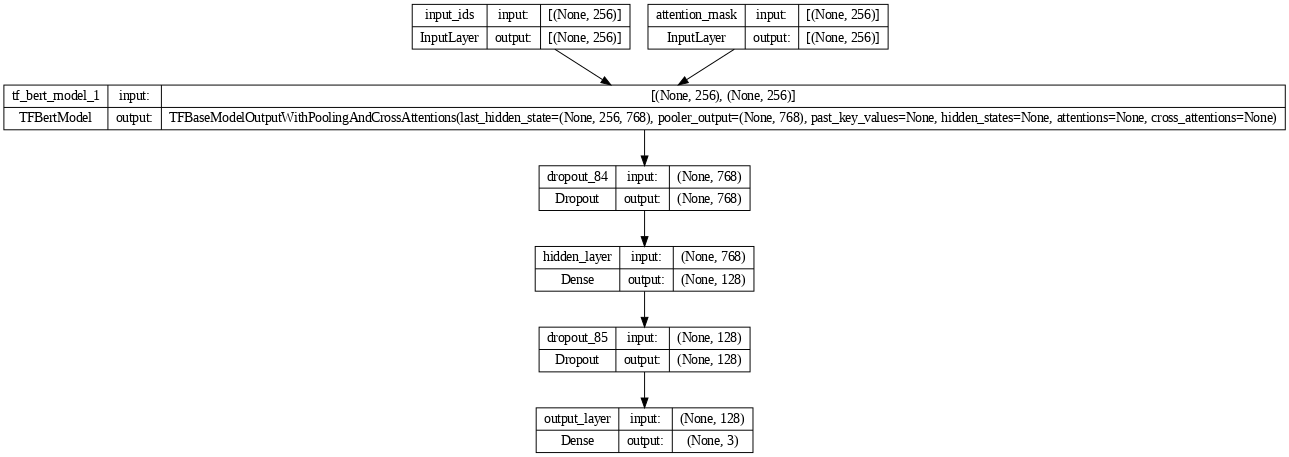
\includegraphics[width = \linewidth]{graphics/FSAB_model.png}
	\caption{The architecture of Financial Sentiment Analysis model using BERT layer}
	\label{fig_FSAB}
\end{figure}
\paragraph{INPUT:}{Our model can predict sentiment of a text of variable length subject to a constraint on the maximum length. Since our model utilizes the BERT language model, our input must be a valid BERT input. FSAB accepts two inputs - input\textunderscore ids and attention\textunderscore mask. To obtain the input\_ids, we first tokenize a text using the BERT-uncased tokenizer. We prepend and appended the tokenized sequence with classification and separator token respectively. Using padding/truncation, we ensure that the input\_ids have length 256. To help BERT distinguish between the actual sequence and padding, we pass the second input, the attention\_mask. }
\paragraph{OUTPUT:}{The FSAB outputs a sequence of three numbers which are the probabilities that the sentiment of the input text is negative, neutral and positive.}
\begin{figure}[h]
	\centering
	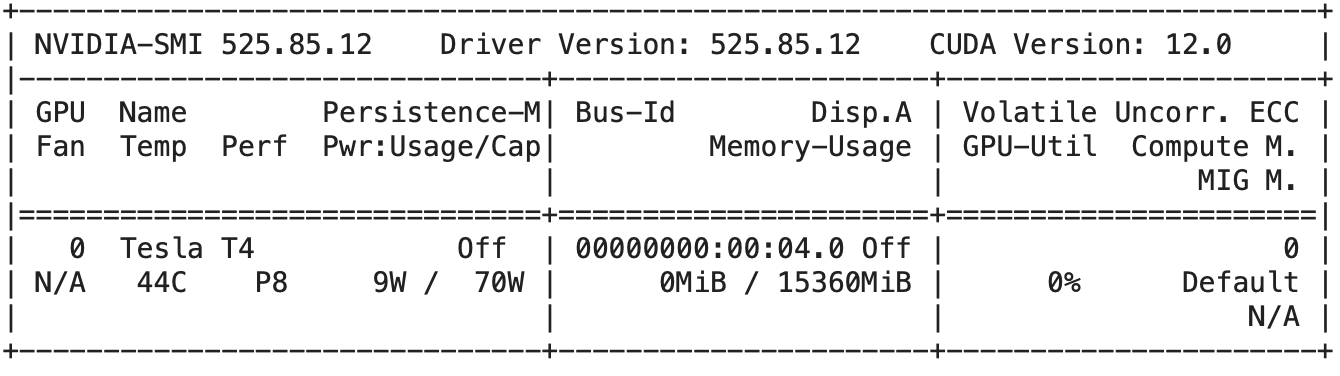
\includegraphics[width = 0.75\linewidth]{graphics/gcolab_runtime.png}
	\caption{NVIDIA System Manager Interface output}
	\label{fig_gcolabruntime}
\end{figure}
\paragraph{TRAINING:} {The model is trained on the Financial Phrasebank\footnote{labeled dataset of financial statements available at \href{www.huggingface.co/datasets/financial_phrasebank}{www.huggingface.co/datasets/financial\_phrasebank}} dataset. To train our model efficiently, we used Google Colaboratory with a GPU runtime, see fig. \ref{fig_gcolabruntime}. We split the dataset into train ($75\%$), validation ($12.5\%$) and test data ($12.5\%$). We create TensorFlow datasets to facilitate parallelization. We used SparseCategoricalCrossEntropy as the loss function. See fig. \ref{fig_FSAB_history} for the loss and accuracy curves.}
%\begin{figure}[h]
%	\centering
%	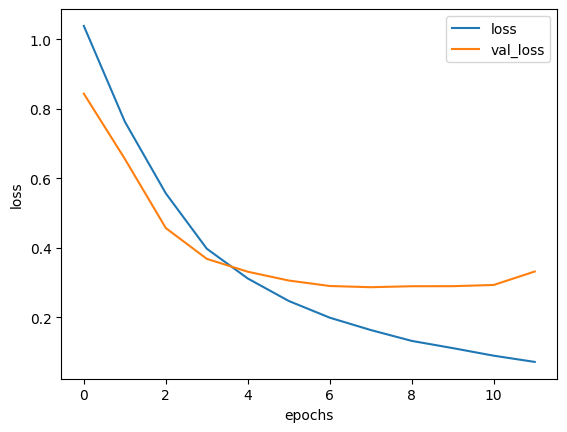
\includegraphics[width = 0.75\linewidth]{graphics/FSAB_loss.png}
%	\caption{Loss curve - FSAB}
%	\label{fig_FSAB_loss}
%\end{figure}
\begin{figure}[h]
	\centering
	\begin{subfigure}{.45\textwidth}
		\centering
			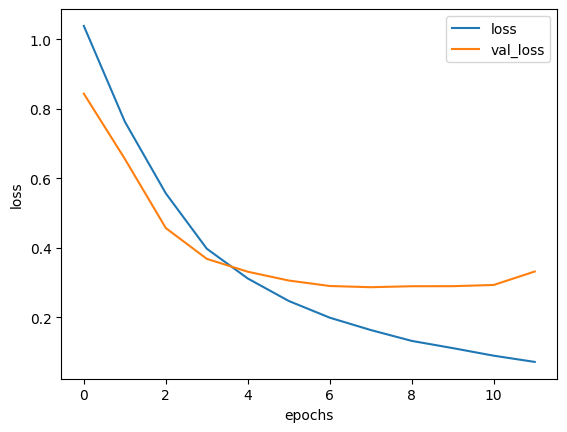
\includegraphics[width = \linewidth]{graphics/FSAB_loss.png}
		\caption{Loss curve - FSAB}
		\label{fig_FSAB_loss}
	\end{subfigure}
	\begin{subfigure}{.45\textwidth}
		\centering
	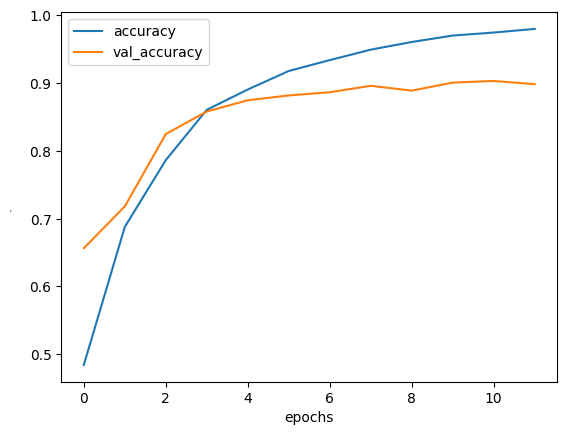
\includegraphics[width = \linewidth]{graphics/FSAB_accuracy.png}
	\caption{Accuracy curve - FSAB}
	\label{fig_FSAB_accuracy}
\end{subfigure}
\caption{FSAB loss and accuracy curves}
\label{fig_FSAB_history}
\end{figure}

\subsection{Performance}
The FSAB model correctly classified the input text with an accuracy close to $95\%$. The probability that the model classified an input of negative sentiment as positive and vice-versa is around $2.5\%$. See table \ref{tab_confusion_matrix} for the confusion matrix on test data.
\begin{table}[h!]
	\centering
	\begin{tabular}{|c|c|c|c|}
		\hline
		& Negative & Neutral & Positive \\
		\hline
		Negative & 49 & 2 & 0\\
		\hline
		Neutral & 2 & 248 & 4\\
		\hline
		Positive & 4 & 6 & 107\\
		\hline
	\end{tabular}
	\caption{Confusion Matrix}
	\label{tab_confusion_matrix}
\end{table}
The trained model can now be used to predict the sentiment of a financial text. For example, running our model on the text `the profit declined by 50\% compared to last year' yields a negative sentiment probability of around 99.4\%. On the other end of the spectrum, the text `the profit in 2023 was 200\% higher than that in 2022' yields a positive sentiment probability of 99.7\%.




\section{Stock price prediction models}\label{sec_stock}
In this section we will develop three models to predict daily stock prices using historical data. Our time series model will predict the next day closing price using past closing prices. The description of the three models are as follows.
\begin{enumerate}
	\item Moving Averages Models - We will use past 5 data points to predict the stock price. We experiment both with simple moving averages (SMA) and exponential moving averages (EMA). In SMA the all past values are given equal weights, while in EMA, average is computed by giving larger weights to recent data points in the time series.
	\item Recurrent Neural Network - In the second model, we will construct a recurrent neural network to predict the stock prices.
	\item Recurrent Neural Network with sentiments - In this model, we will construct a recurrent neural network and also utilize daily sentiments to predict the stock prices. To obtain sentiments data, we will webscrape Google news for each day and compute the sentiment using FSAB described above. 
\end{enumerate}

\subsection{Moving average models}
\begin{figure}[h]
	\centering
	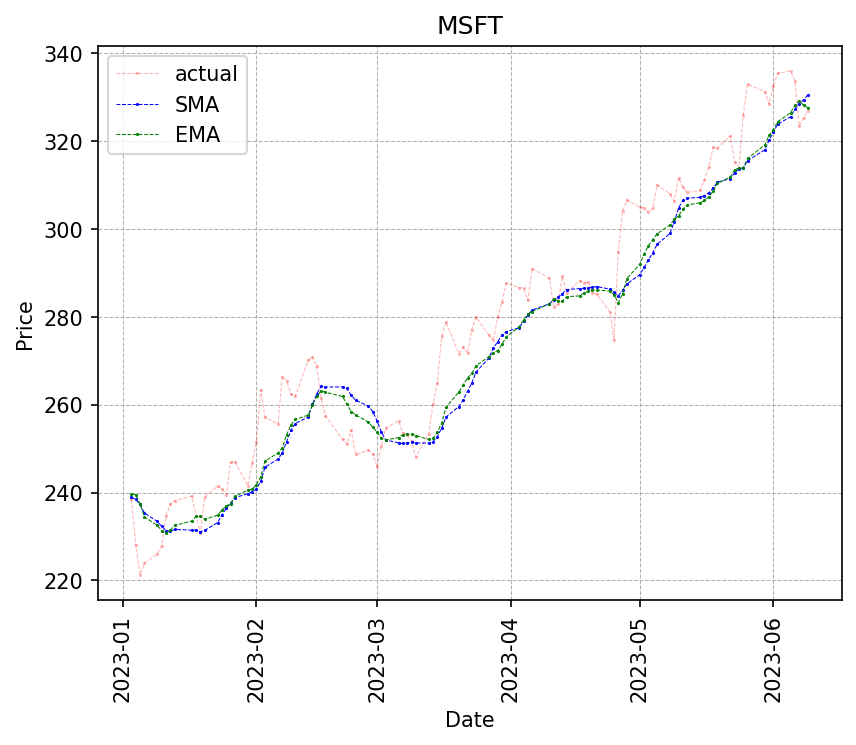
\includegraphics[width = 0.75\linewidth]{graphics/moving_averages.png}
	\caption{Stock price prediction - Moving average models}
	\label{fig_moving_averages}
\end{figure}
In the simple moving average model, the stock price at next time instance is predicted to be the average of last $N$ stock prices.
\begin{equation}
	SMA_{N+1} = {1\over N} \sum\limits_{i = 1}^{N} S_i
\end{equation}
Whereas, in the case of exponential moving average the prediction is
\begin{equation}
EMA_{N+1} = {2\over N+1} S_N + {N-1 \over N+1} \, EMA_{N} 
\end{equation}
We predict the closing price of Microsoft (MSFT) with $N=5$. The root mean square error for the simple moving average model and the exponential moving average is 9.25 and 8.48 respectively. Fig. \ref{fig_moving_averages} shows the actual stock price and the predictions using moving averages.




\subsection{Recurrent Neural Network}
A Recurrent Neural Network is often useful for modeling time series data. To model the stock price, we first assume that the stock price receives contribution from a deterministic and a stochastic term. 
\begin{equation}
	S(t) = S_0 \, e^{\alpha t} + \eta(t),
\end{equation}
where the first term is a deterministic drift and encodes the long time behavior, and the second term is a stochastic contribution that depends on short time market features. We estimate $S_0$ and $\alpha$ using a linear fit of $\log(S)$ as a function of $t$, see fig. \ref{fig_drift}. We model $\eta$ using a recurrent neural network. 
\begin{figure}[h]
	\centering
	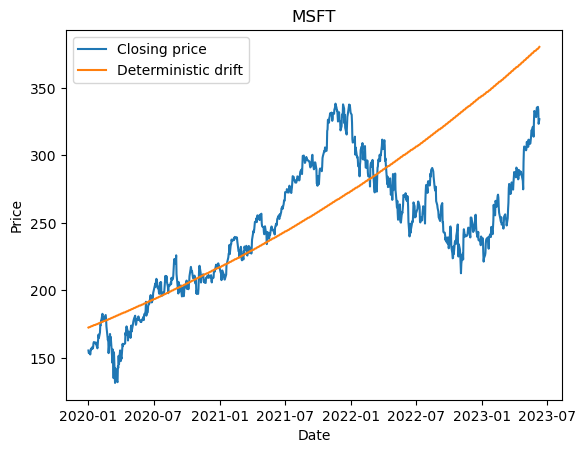
\includegraphics[width = .75\linewidth]{graphics/drift.png}
	\caption{Long term behavior of stock price}
	\label{fig_drift}
\end{figure}
\paragraph{Model:}{After experimenting with the model architecture, we determined that the best performance was achieved when last 5 stock prices were used to predict the future stock price. To counter against the vanishing gradient problem, we initially experimented with an LSTM (Long Short Term Memory) model. However, since only last 5 data points were used for prediction, we found that a recurrent neural network performed better than LSTM. To prevent over fitting, we used L2-Kernel regularization, dropout and recurrent dropout. See fig. \ref{fig_simplernn_model} for model architecture.}
\begin{figure}
	\centering
	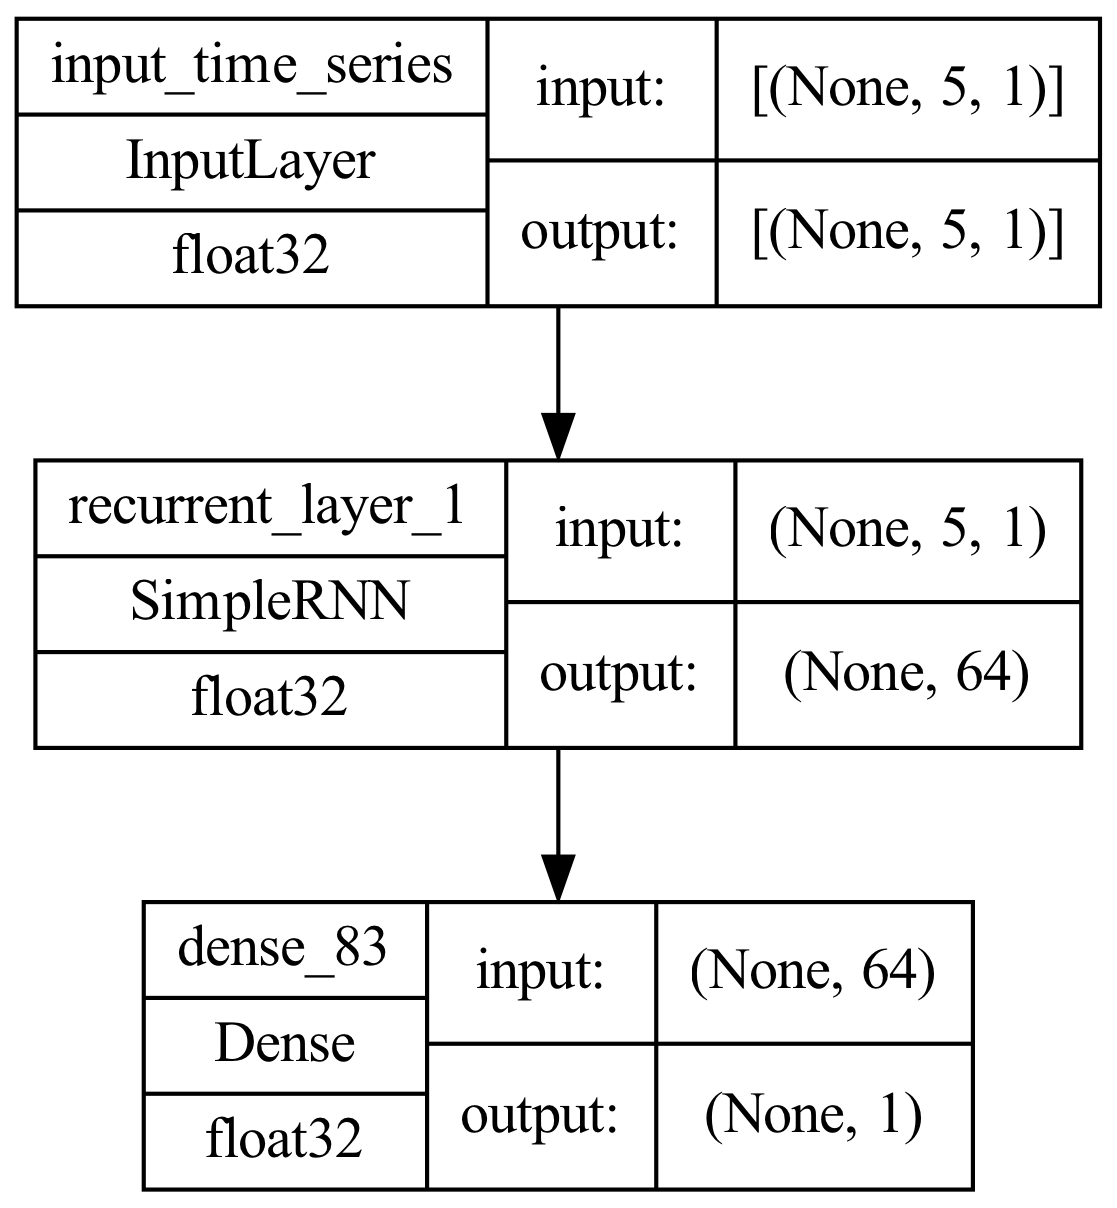
\includegraphics[width=.25\linewidth]{graphics/simplernn_model}
	\caption{Architecture of model for predicting stock price using a recurrent neural network}
	\label{fig_simplernn_model}
\end{figure}
\paragraph{Training and performance:}{The model was trained on daily closing stock price of Microsoft (MSFT) from January 2020 to December 2022 and performance was evaluated on stock prices from January to June 2023\footnote{Recall that we use RNN to predict $\eta$. For a better fitting of the model, we scaled the stock prices using StandardScaler from sklearn. To evaluate performance, we rescaled the output of our model and added the deterministic drift to obtain the final stock price.}. The root mean squared error on test data was close to 5.9, which is  around 35\% lower than moving average models. Fig. \ref{fig_simplernn} shows the plot of actual stock prices and predictions of RNN model.}
\begin{figure}[h]
	\centering
	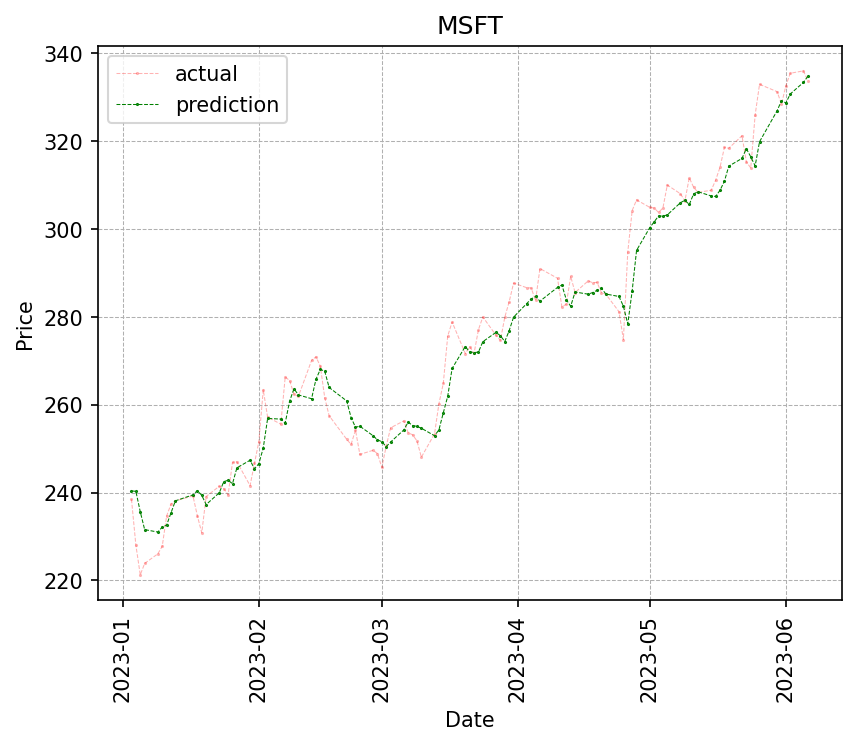
\includegraphics[width = 0.75\linewidth]{graphics/simplernn.png}
	\caption{Stock price prediction - Recurrent Neural Network}
	\label{fig_simplernn}
\end{figure}

\subsection{Recurrent Neural Network with sentiment}
In the final model of this project, we attempt to combine the recurrent neural network with daily sentiment data to predict the stock price. We compute the sentiment of webscraped google news headlines with search term ``microsoft news''. We used the FSAB model, see sec. \ref{sec_FSAB}, to compute the probabilities that the sentiment is negative, neutral and positive. We then create a dataset with stock prices and sentiments. Our model takes past 5 stock prices and the sentiments as data to predict the future stock price. We now elaborate on the various steps involved.
\paragraph{Webscraping:}{We used the BeautifulSoup library to automate collection of Google news headlines. We searched Google news website for articles on ``microsoft news'' published on a given date. We scraped the headlines from the first page of search results, appended the headlines to a file and then varied the date. This automated process allowed us to collect top news headlines pertaining to Microsoft on each day from January 2020 to June 2023.  }
\paragraph{Sentiment analysis:}{We used the trained FSAB model, sec. \ref{sec_FSAB}, to obtain the sentiments of the headlines collected earlier. Once again, we saved the sentiment data to a file for later use.}
\paragraph{Model:}{Our model takes the last 5 stock prices and average sentiment probabilities as input and outputs the prediction for next stock price. It works in two steps. First, our model uses a recurrent neural network with the last 5 stock prices as input and gives an intermediate prediction for the stock price. In the next step, the model uses this intermediate prediction and the sentient probabilities to output the final prediction for the stock price. Once again, we use various regularization techniques discussed earlier to prevent over fitting. The model architecture is shown in fig. \ref{fig_model}.}
\begin{figure}
	\centering
	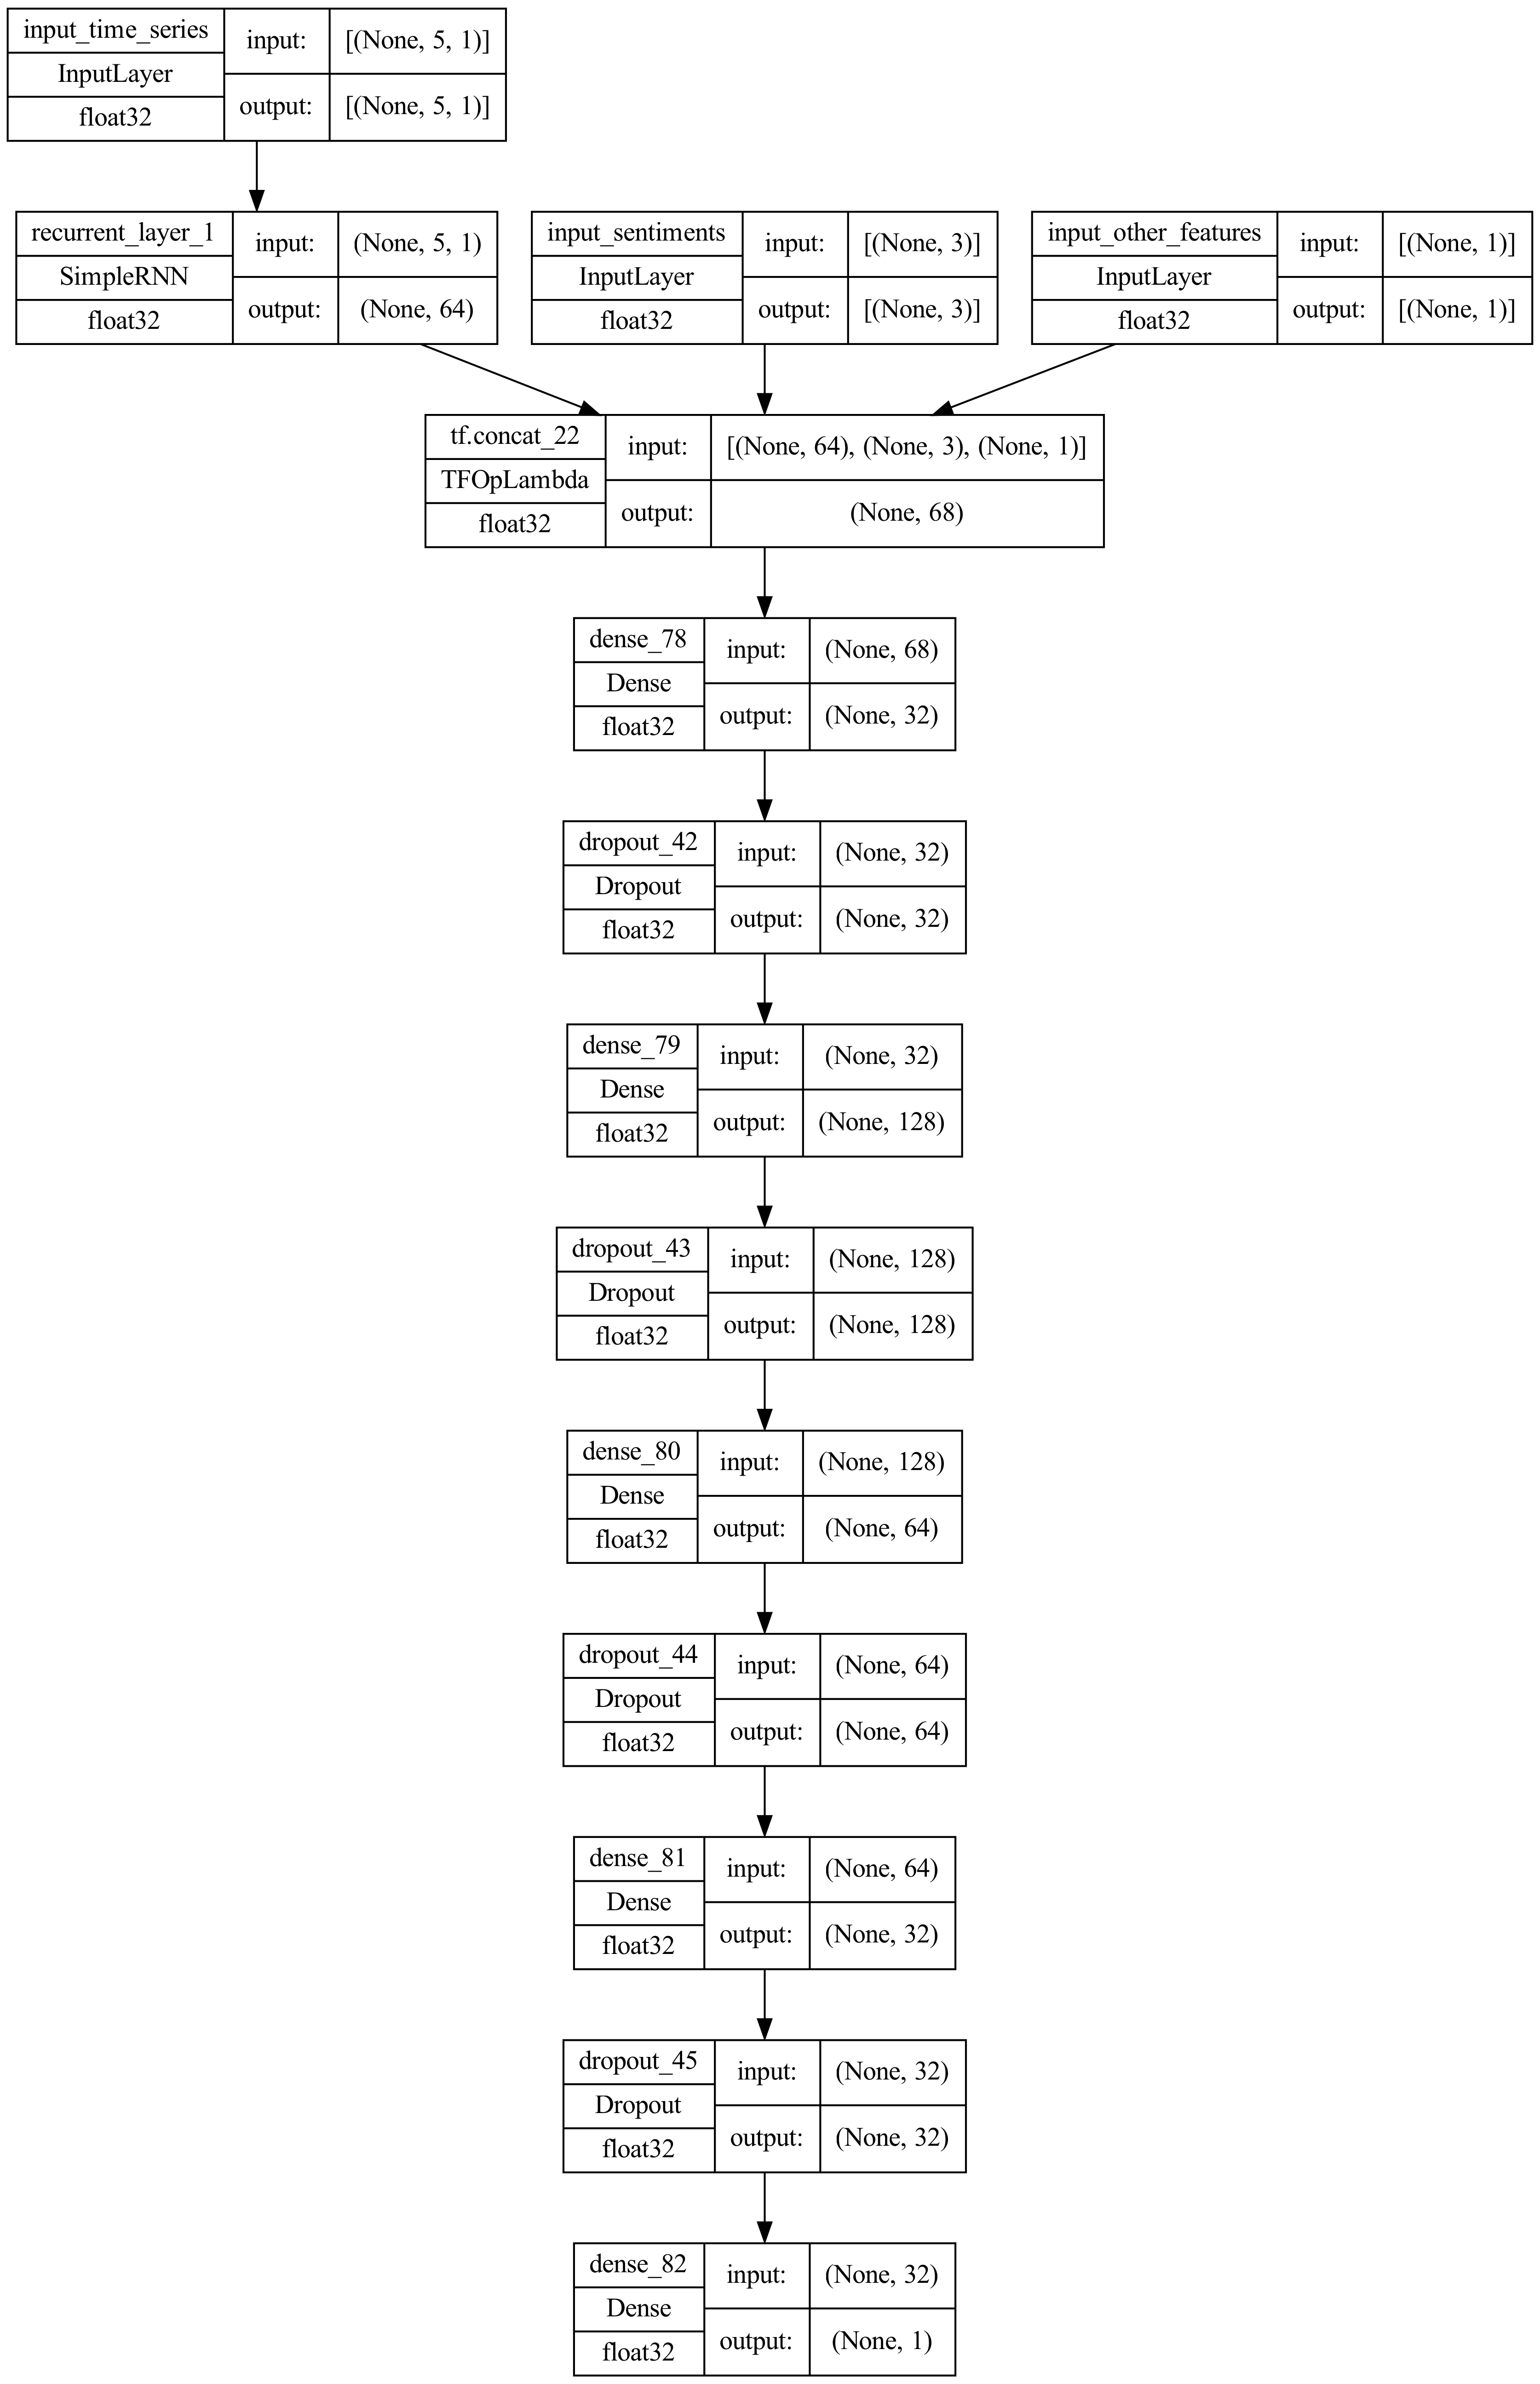
\includegraphics[width = 0.75\linewidth]{graphics/model.png}
	\caption{Architecture of the RNN with sentiment model. This model can be readily expanded to include more features. However, for the purpose of this project, we only work with closing price and sentiments.}
	\label{fig_model}
\end{figure}
\paragraph{Training and performance:}{As with earlier models, this model was trained on daily closing stock price of Microsoft (MSFT) from January 2020 to December 2022 and performance was evaluated on stock prices from January to June 2023. We found that there was negligible correlation between sentiment and stock prices, see fig. \ref{fig_sentiment_stock_correlation}. The Pearson correlation coefficient between stock price movement and sentiment was less than 0.1. However, the correlation coefficient became -0.37, for instance, when we restricted to negative sentiment probability larger than 0.5. It appears that strong sentiment does seem to be mildly correlated with stock price movement. However, it is unclear if including sentiments would enhance the performance.
\begin{figure}[h]
		\centering
		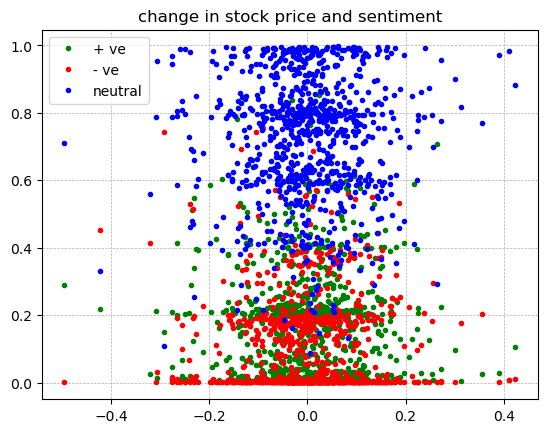
\includegraphics[width = .75\linewidth]{graphics/sentiment_stock_correlation.png}
		\caption{Sentiment probabilities and daily closing stock price movement}
		\label{fig_sentiment_stock_correlation}
\end{figure}
In fact, we found that the root mean squared error for this model (on test data) was approximately 8.13. This model performed better than the moving average models, but worse than the simple RNN model. See fig. \ref{fig_sentimentrnn}}.
\begin{figure}[h]
	\centering
	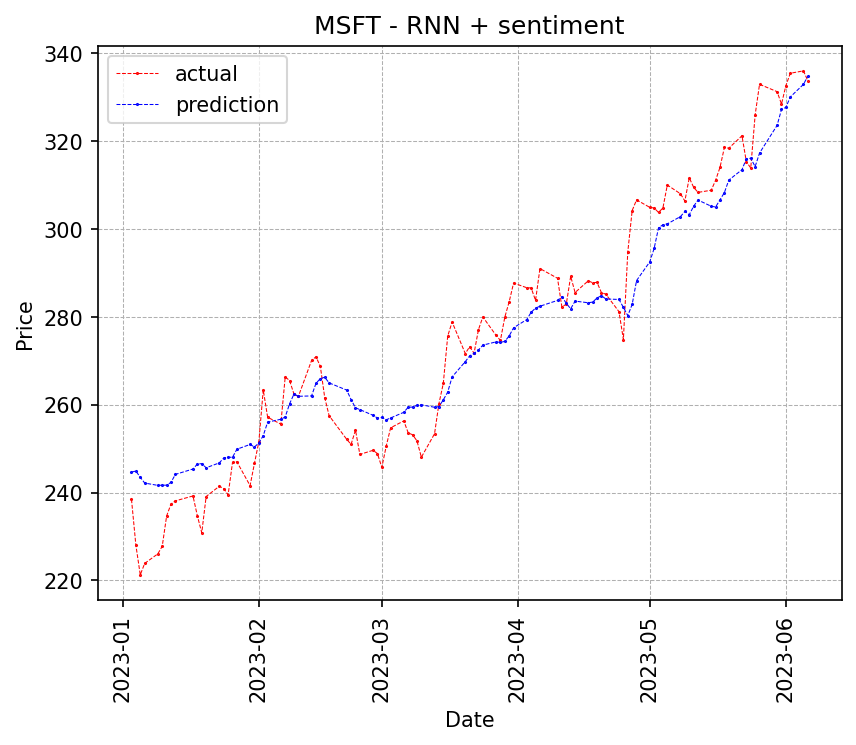
\includegraphics[width = .75\linewidth]{graphics/sentimentrnn.png}
	\caption{Stock price prediction - RNN based model with daily sentiments}
	\label{fig_sentimentrnn}
\end{figure}

\section{Summary and discussions}
In this project we analyzed the utility of machine learning techniques in stock price prediction. We developed a machine learning model to predict the sentiment of a financial text. We also developed several models to predict the daily closing price of a particular stock. We found that our Neural Network based model improved stock price prediction by about 35\%. 
\subsection{Financial sentiment analysis}
To predict the sentiment of a financial text, we added a classification layer to the pre-trained Bidirectional Encoder Representations from Transformers (BERT) language model. We fine-tuned our model (FSAB) on the Financial Phrasebank database and evaluated the performance. We found that our model's accuracy on test data was close to 95\%. See sec. \ref{sec_FSAB} for further details. We later used this model to predict the sentiment of news headlines pertaining to the stock of interest.
\subsection{Stock price prediction}
In sec. \ref{sec_stock}, we studied the performance of 4 models to predict the stock price. The first two models were Simple Moving Average and Exponential Moving Average models. The third model implemented a Recurrent Neural Network (RNN) while the final model also incorporated sentiment data apart from RNN. To obtain sentiment data, we webscraped Google news using the BeautifulSoup library. For a comparison of the performance of these models, see tab \ref{tab_comparison}. All of the models used last 5 data points to make predictions.
\begin{table}[h!]
	\centering
	\begin{tabular}{|c|c|c|c|c|}
		\hline
		Model & SMA & EMA & RNN & RNN + sentiment \\
		\hline
		RMSE & 9.25 & 8.48 & \textbf{5.85} & 8.13 \\
		\hline
	\end{tabular}
	\caption{Comparison of stock prediction models}
	\label{tab_comparison}
\end{table}
At first glance, it may be surprising that the model with sentiment doesn't yield the best performance. However, this can be attributed to the quality of data collected for sentiment analysis as well as the low frequency of stock price data. 
\subsection{Future directions}
It would be interesting to explore the role of other data, such as fundamental data and macroeconomic data, in stock price prediction since our model can be readily modified to accommodate additional features. Another direction is to study the performance of various models at a different time scale. For instance, one can try to predict stock prices at higher frequency, say every minute or even every second. It is reasonable that RNN model might yield even better results in shorter timescales.  Finally, it would be interesting to explore the relation between sentiment and stock price movement at different timescales. However, this require collection of more frequenct and robust news/opinions data which is beyond the scope of this work.

%\bibliographystyle{JHEP}
%
%\bibliography{references}
\end{document}